\section{Firefly Algorithm}

The firefly algorithm is a nature-inspired, meta-heuristic optimisation
algorithm. The algorithm, presented by Yang et al., is derived from the
flashing behaviour of fireflies. We will not go into biological details of this
phenomena, but instead will focus on the simplified set of rules that
artificial fireflies follow, as presented in \cite{firefly}. First, any firefly
is attracted by any other firefly. Second, the attraction depends on the
brightness of the fireflies, and last, the attraction decreases with increasing
distance.  Each firefly represents one solution to the optimisation problem. We
initialise the fireflies randomly over the search space. The brightness of a
firefly is determined by the firefly's error (or its reciprocal, depending if
we seek for maximisation or minimisation). At each iteration each firefly
moves a little step into the direction of each other firefly that has a higher
brightness. The formula of the movement is given as:

\begin{equation}
    \mathbf{x_i} = \mathbf{x_i} + \beta_0 e^{-\gamma r_{ij}^2} + \alpha (rand - \frac{1}{2})
\end{equation}

where $\mathbf{x_i}$ is the current position, $\beta_0$ is the attractiveness
at distance 0, $\gamma$ is the absorption coefficient, $r_{ij}$ is the distance
between the two fireflies, $\alpha$ is a randomisation parameter, and $rand$ a
random number between 0 and 1.

\subsection{Experiments}

In this section we compare our implementation of the firefly algorithm to the
reference evolutionary algorithm. For our tests we initialised 50 fireflies and
optimise over 275 iterations. We used following parameters for all experiments:
$\alpha = 0.001$, $\beta_0 = 1$, and $\gamma = 0.05$.

As table \ref{tab:firefly_vs_ea} and figure \ref{fig:firefly_vs_ea} are
showing, the firefly algorithm outperforms the reference evolutionary algorithm
on the DTLZ1 problem, even with a smaller number of evaluations and a shorter
run-time. We adapted the number of iterations we used in the firefly algorithm,
such that the number of evaluations is roughly the same as in the reference
algorithm, to allow for a fair comparison. We averaged the results of 10
subsequent runs and give the standard deviation in table
\ref{tab:firefly_vs_ea}. The number of evaluations done in the firefly
algorithm is also averaged over 10 runs, because as opposed to the reference
algorithm, the number of evaluations is not constant in each iteration.

\begin{table}[H]
  \centering
   \begin{tabular}{|c c c c|}
     \hline
     \textbf{Optimizer} & \textbf{Error} & \textbf{Evaluations} & \textbf{Runtime [ms]} \\
     \hline
     Firefly Algorithm & $781.63 \pm 42.28$ & 227912 & 8.39 \\
     Reference Evolutionary Algorithm & $3003.58 \pm 87.35$ & 250000 & 24.53 \\
     \hline
  \end{tabular}
  \caption{Minimal errors after the given number of evaluations produced by optimisers on the DTLZ1 problem. Results are averaged over 10 subsequent runs.}
  \label{tab:firefly_vs_ea}
\end{table}

\begin{figure}
  \centering
  \begin{subfigure}{.5\textwidth}
    \centering
    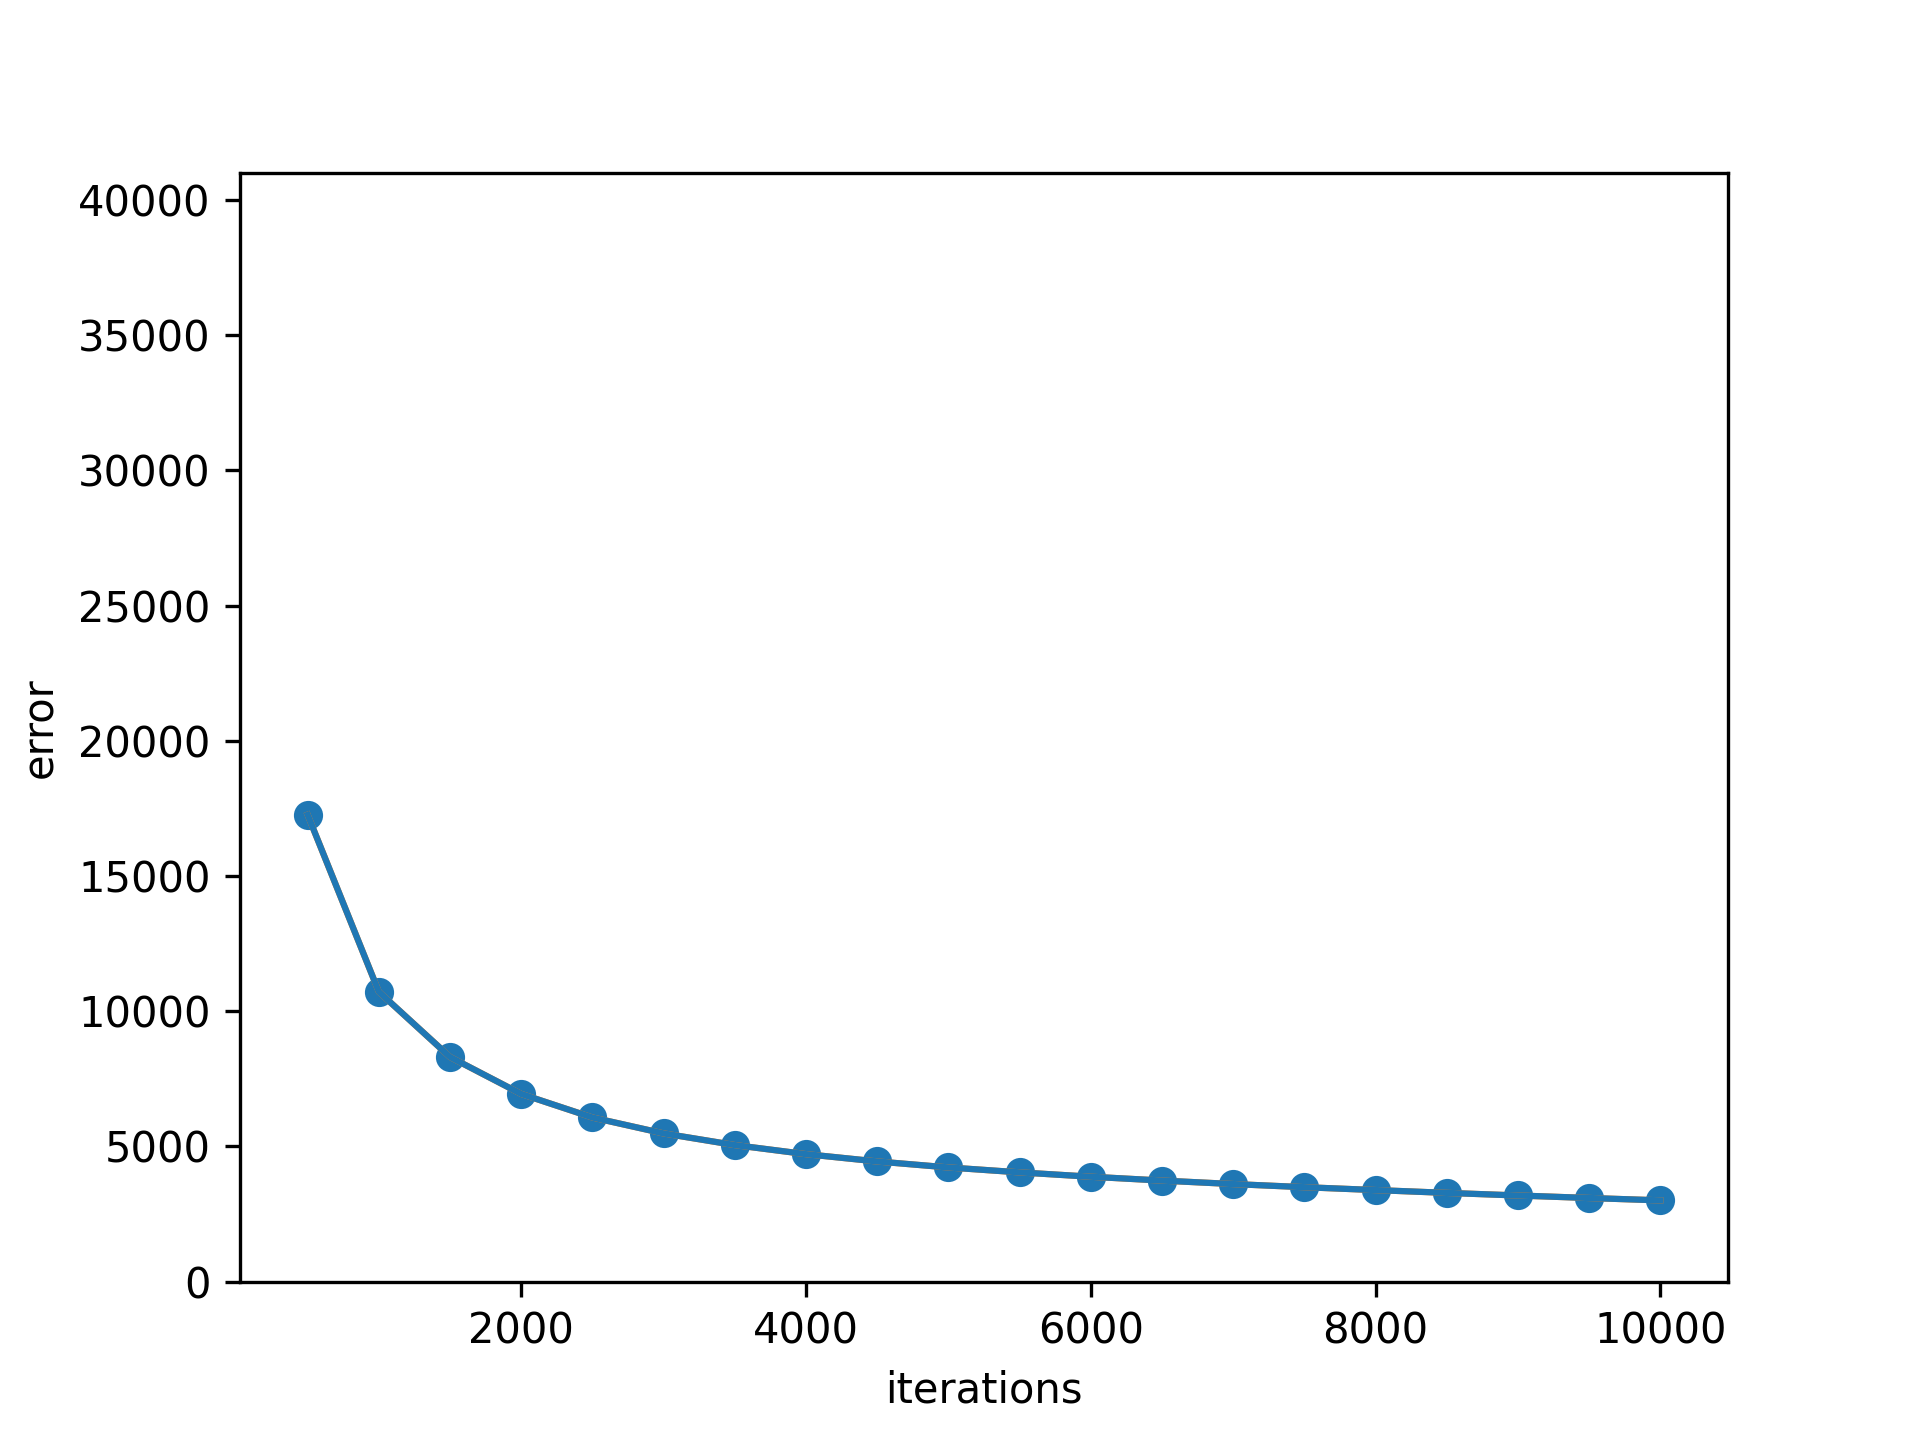
\includegraphics[width=0.75\linewidth]{assets/reference.png}
    \caption{Error over iterations using the reference evolutionary algorithm.}
    \label{fig:sub1}
  \end{subfigure}%
  \begin{subfigure}{.5\textwidth}
    \centering
    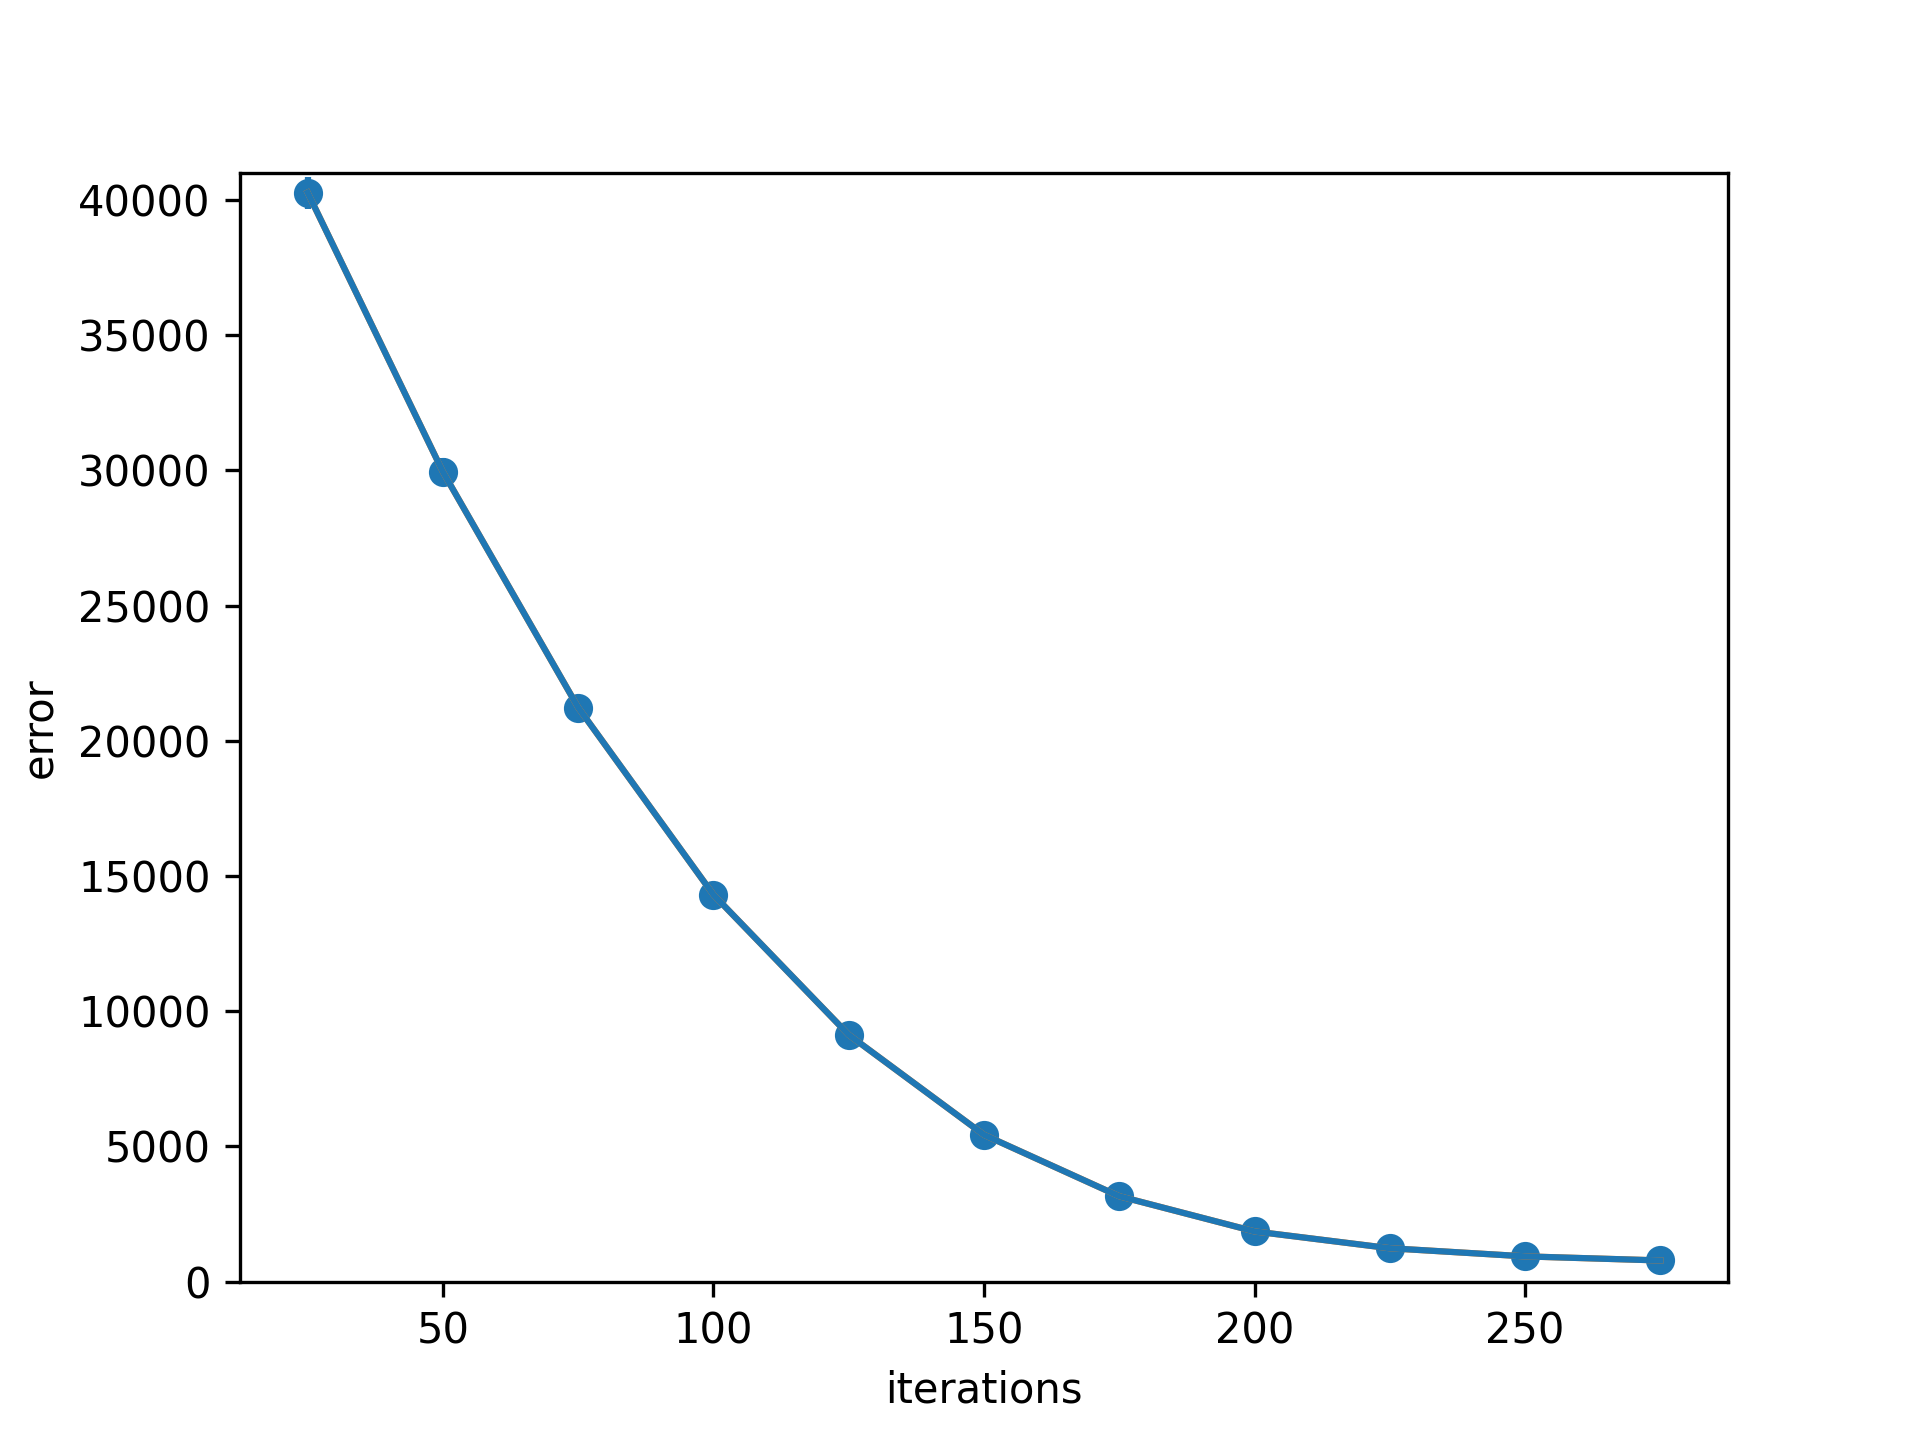
\includegraphics[width=0.75\linewidth]{assets/firefly.png}
    \caption{Error over iterations over using the firefly algorithm.}
    \label{fig:sub2}
  \end{subfigure}
  \caption{Comparison of firefly and evolutionary algorithm on the DTLZ1 problem. \ref{tab:firefly_vs_ea}.}
  \label{fig:firefly_vs_ea}
\end{figure}

